\documentclass[12pt]{article}
\usepackage[pdftex]{graphicx}
\usepackage{amsfonts}
\usepackage[italian]{babel}
\usepackage{graphicx}
\usepackage{color}
\usepackage{multirow,bigdelim}
\usepackage{relsize}
\usepackage{fdsymbol}
\usepackage{mdframed}

\definecolor{grey}{rgb}{0.3,0.3,0.3}
\definecolor{verylightgray}{rgb}{.97,.97,.97}
\definecolor{lightred}{rgb}{1,.70,.70}

\usepackage{listings, framed}
\lstset{
  language=Java,
  showstringspaces=false,
  columns=flexible,
  basicstyle={\small\ttfamily},
  frame=none,
  numbers=none,
  keywordstyle=\bfseries\color{grey},
  commentstyle=\itshape\color{red},
  identifierstyle=\color{black},
  stringstyle=\color{blue},
  numberstyle={\ttfamily},
%  breaklines=true,
  breakatwhitespace=true,
  tabsize=3,
  escapechar=|
}

\mdfsetup{font=\scriptsize}

\def\codesize{\smaller}
\def\<#1>{\codeid{#1}}
\newcommand{\codeid}[1]{\ifmmode{\mbox{\codesize\ttfamily{#1}}}\else{\codesize\ttfamily #1}\fi}

%****************enlarge layout
\textheight     243.5mm
\topmargin      -20.0mm
\textwidth      500pt
\hoffset        -80pt
%*****************theorems and such
\newcounter{esnu}
\newenvironment{esercizio}{\medskip \noindent {\bf Esercizio\addtocounter{esnu}{1} \arabic{esnu}}}{}
\pagestyle{empty}
\newcommand{\liff}{\mathrel{\leftrightarrow}}   % Logical IFF Symbol
\newcommand{\metaiff}{\Longleftrightarrow}      %iff in metatheory

\begin{document}

\begin{center}
  \textbf{Esame di Programmazione II, 16 febbraio 2024}\\
  (si consegni \texttt{PrefixMap.java})
\end{center}

\emph{
Si crei un progetto Eclipse e
il package \<it.univr.prefix>. Si copino al suo interno
le classi del compito.
Non si modifichino le dichiarazioni dei metodi e delle classi. Si possono definire altri campi,
metodi o costruttori non richiesti dal compito, ma devono essere \<private>. Si possono definire altre classi,
che in tal caso vanno consegnate.
La soluzione che verr\`a consegnata dovr\`a compilare,
altrimenti non verr\`a corretta.}

\vspace*{2ex}

Un \emph{albero di prefissi} \`e un'implementazione di una mappa
da stringhe a valori (possibilmente \<null>) di tipo \<E>.
Il seguente \<Main>
crea un albero di prefissi per valori di tipo \<Integer>, lo popola
con dei legami chiave/valore (con il metodo \<put>) che poi rilegge
(con il metodo \<get>):

\begin{lstlisting}[language=Java]
public class Main {
  public static void main(String[] args) {
    PrefixMap<Integer> pm = new PrefixMap<Integer>();
    pm.put("hello", 13);            pm.put("computer", 17);        pm.put("computee", 19);
    pm.put("courage", 41);          pm.put("alliance", 17);        pm.put("help", 78);
    pm.put("computed", 91);         pm.put("courage", 42);         pm.put("", 11);
    pm.put("alliances", null);
    System.out.println("computer -> " + pm.get("computer"));
    System.out.println("computed -> " + pm.get("computed"));
    System.out.println("computee -> " + pm.get("computee"));
    System.out.println("hello -> " + pm.get("hello"));
    System.out.println("help -> " + pm.get("help"));
    System.out.println("hel -> " + pm.get("hel")); // null perche' non c'e'
    System.out.println("helpo -> " + pm.get("helpo")); // null perche' non c'e'
    System.out.println(" -> " + pm.get(""));
    System.out.println("alliance -> " + pm.get("alliance"));
    System.out.println("alliances -> " + pm.get("alliances")); // null perche' non c'e'
    System.out.println("courage -> " + pm.get("courage"));
    System.out.println("computers -> " + pm.get("computers")); // null perche' non c'e'
    System.out.println(pm); // stampa la struttura dell'albero
    pm.put(null, 113); // va in eccezione
  }
}
\end{lstlisting}
%
La sua esecuzione dovr\`a stampare:

\begin{mdframed}[backgroundcolor=lightred]
  {\small\begin{verbatim}
computer -> 17
computed -> 91
computee -> 19
hello -> 13
help -> 78
hel -> null
helpo -> null
 -> 11
alliance -> 17
alliances -> null
courage -> 42
computers -> null

        "lo": 13
    "hel"
        "p": 78
            "r": 17
        "mpute"
            "e": 19
            "d": 91
    "co"
        "urage": 42
""
        "": 17
    "alliance"
        "s": null
    "": 11

Exception in thread "main" java.lang.NullPointerException: null keys are not allowed
\end{verbatim}}
\end{mdframed}
%
La stampa termina con la struttura interna dell'albero di prefissi,
che graficamente possiamo disegnare meglio come segue (la radice \`e a
sinistra e le foglie sono a destra; in questo caso la radice
contiene il prefisso stringa vuoto, ma non \`e detto che sia sempre cos\'{\i}):
%
\begin{center}
  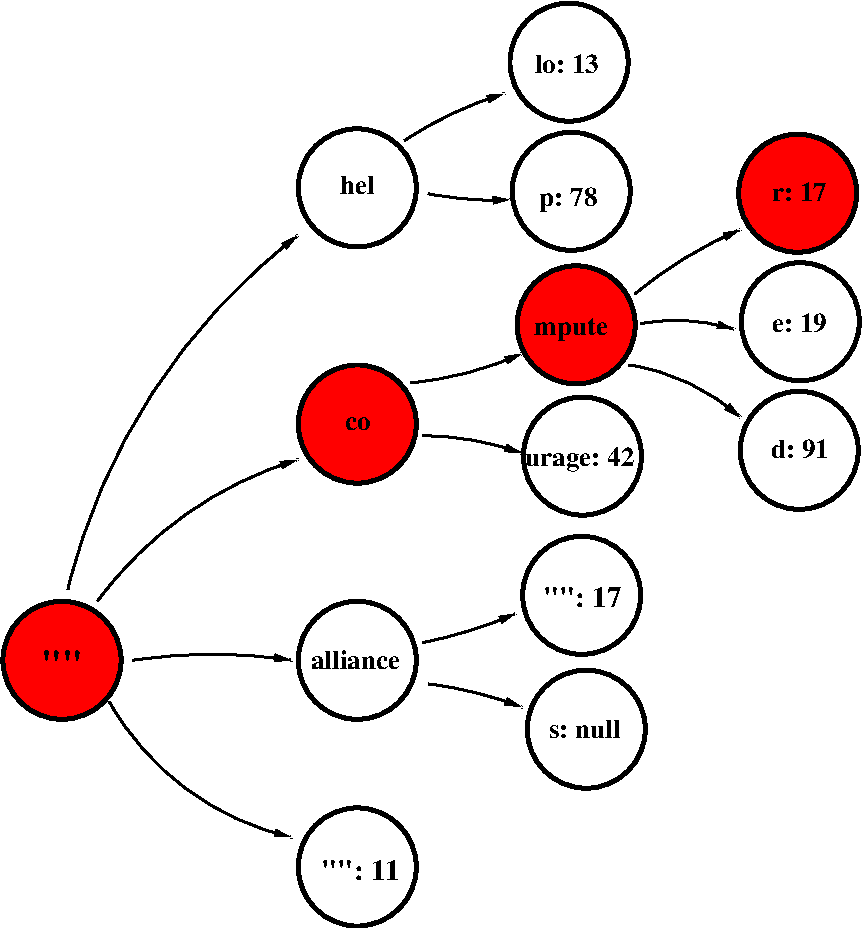
\includegraphics[width=0.6\textwidth]{tree}
\end{center}
%
Per ogni cammino dalla radice a una foglia, concatenando i prefissi sul cammino,
si ottiene una chiave legata al valore nella foglia. Per esempio,
abbiamo evidenziato in rosso un percorso che mostra come la stringa
\<computer> sia associata al valore 17. Si noti che i figli
di un nodo hanno sempre prefissi mutuamente esclusivi. Per esempio,
i figli del nodo contenente \<co> hanno prefissi \<mpute> e \<urage>,
che non iniziano con la stessa lettera. Questo semplifica la ricerca
del valore legato a una chiave stringa, perch\'e c'\`e solo un percorso
in cui ci si pu\`o muovere durante la ricerca di una chiave
dalla radice verso le foglie.

\vspace*{2ex}\textbf{Esercizio 1 ($2$ punti).}
Il metodo \<put> di \<PrefixMap> \`e gi\`a scritto e funzionante: lo si completi
facendogli generare una \<NullPointerException>, con messaggio
\<null keys are not allowed>, nel caso in cui la chiave \<key> fosse \<null>.

\vspace*{2ex}\textbf{Esercizio 2 ($14$ punti).}
Si completi il metodo \<get> di \<PrefixMap> aggiungendo
un metodo pubblico ricorsivo sui nodi, ridefinito per i nodi interni e i nodi foglia,
come \`e stato gi\`a fatto per \<put>.
Intuitivamente, se si cerca il valore legato a una chiave $k$, a partire da un
nodo $n$, allora ci sono due casi:
%
\begin{enumerate}
\item $n$ \`e una foglia: l'unica possibilit\`a \`e che $k$ sia il prefisso
  memorizzato dentro $n$, nel qual caso il valore cercato \`e quello
  scritto dentro la foglia $n$;
\item $n$ \`e un nodo interno: se $k$ inizia con il prefisso memorizzato
  dentro $n$, allora si elimina tale prefisso dall'inizio di $k$, ottenendo
  $k'$. Poi si prova a cercare $k'$ a partire dai figli di $n$, ricorsivamente.
  Se una chiamata ricorsiva trova un valore, allora la ricerca ha avuto
  successo e si ritorna tale valore.
  Altrimenti si ritorna \<null> (la chiave non \`e stata trovata).
\end{enumerate}

\vspace*{2ex}\textbf{Esercizio 3 ($15$ punti).}
Si completi il metodo \<toString> di \<PrefixMap> in modo da fargli
ritornare una
stringa che descrive la struttura dell'albero (si veda l'esempio
di stampa alla pagina precedente). Occorrer\`a
aggiungere un metodo pubblico ricorsivo sui nodi,
ridefinito per i nodi interni e i nodi foglia,
come \`e stato gi\`a fatto per \<put>.
Intuitivamente, se si vuole trasformare in stringa l'albero radicato in un
nodo $n$, allora ci sono due casi:
%
\begin{enumerate}
\item $n$ \`e una foglia con dentro un prefisso $p$ e un valore $v$:
  si ritorna la stringa $p:v$, pi\`u un'andata a capo.
\item $n$ \`e un nodo interno con $f$ figli: si trasformano ricorsivamente
  in stringhe i primi $\frac{f}{2}$ figli, concatenandole; si concatena
  il prefisso memorizzato dentro $n$;  si trasformano ricorsivamente
  in stringhe i restanti $f-\frac{f}{2}$ figli, concatenandole; si ritorna
  la concatenazione complessiva.
\end{enumerate}
%
Quanto si concatenano le stampe dei figli, occorre fare un'indentazione
di quattro spazi verso destra, come nell'esempio
di stampa alla pagina precedente. Il suggerimento \`e di non preoccuparsi
di tale indentazione, in una prima versione, e di aggiungerla successivamente,
se il risultato sembra corretto. Si ricorda che \`e stato fatto
in laboratorio un esempio simile di indentazione durante una discesa ricorsiva.

\end{document}
